% ============================================================
% Baseball2Vector — CVPR Workshop (CVsports) style draft
% ------------------------------------------------------------
% HOW TO USE ON OVERLEAF:
%  1) Start from the official CVPR template project
%     (search "CVPR 2026" in Overleaf templates), which provides
%     cvpr.sty and the review/final options.
%  2) Replace the main .tex with this file.
%  3) Copy the three revised figures into a
%     figures/ folder in the Overleaf project:
%       - figure1_alignment_revised.pdf
%       - figure2_profile_diversity_revised.pdf
%       - figure3_delta_association_revised.pdf
%  Numbers are traceable to the adjacent results/ and tables/
%  directories in the isolated final-academic-revision workspace.
% ============================================================

\documentclass[10pt,twocolumn,letterpaper]{article}

% --- CVPR template package (from the official template project) ---
\usepackage[pagenumbers]{cvpr}   % use [review] for the review version

\usepackage{graphicx}
\usepackage{amsmath,amssymb}
\usepackage{booktabs}
\usepackage{multirow}
\usepackage{xurl}
\usepackage[pagebackref,breaklinks,colorlinks]{hyperref}

\def\paperID{****}
\def\confName{CVPR Workshop (CVsports)}
\def\confYear{2026}

\begin{document}

%%%%%%%%% TITLE
\title{Baseball2Vector: An Interpretable Five-Dimensional Skill Representation of MLB Position Players}

\author{Jaeseok Choi\\
I2SLAB, Sungkyunkwan University\\
{\tt\small jaeseok.choi@skku.edu}
}

\maketitle

%%%%%%%%% ABSTRACT
\begin{abstract}
Scalar baseball metrics compress qualitatively different player profiles onto one axis. We propose \emph{Baseball2Vector}, a season-level representation of Power, Contact, Plate Discipline, Defense, and Speed on a cohort-relative 20--80-formatted scale. Using 2{,}309 MLB hitter-seasons from 2021--2025 ($\geq$100 PA), we compare three encoders and evaluate the Z-score representation prospectively. In a forecast-safe 2024$\to$2025 test of 358 returning players, B2V-only Ridge obtains MAE 18.03, $R^2=0.280$, and Spearman $\rho=0.508$. It improves MAE over calibrated current-wRC+ Ridge by 1.19 points (95\% paired-bootstrap CI $[0.40,2.01]$); a combined scalar-plus-B2V model likewise improves the scalar-context baseline, although adding current wRC+ to B2V does not improve B2V-context performance. Different players matched on wRC+ and WAR remain farther apart than the same player across adjacent seasons (median standardized distance 1.004 vs.\ 0.714). These results support modest incremental predictive information and interpretable profile diversity, not scouting-grade validity or causal development guidance. Raw-input comparison remains unavailable, and the Defense construction remains unresolved.
\end{abstract}

%%%%%%%%% BODY
\section{Introduction}
\label{sec:intro}

Evaluating and comparing player ability is central to modern baseball. For front offices, accurately gauging a player's ability underpins the decisions that matter most: which prospects to draft or sign, and which players to deploy in which roles. For players themselves, an objective account of where their strengths and weaknesses lie is a prerequisite for targeted development. And for fans, much of the enjoyment of the sport comes from understanding \emph{how} a player is good---which tools carry them---and from counterfactual imagination: ``what if this player added power?'' In all three cases, what is needed is not merely a ranking but a \emph{representation}: a compact, interpretable description of a player that supports comparison, communication, and reasoning.

Existing answers are only partial. Sabermetric composites such as WAR and wRC+ condense a player's contribution into a single number, which is invaluable for ranking but discards profile information: a slugger with poor contact skills and a well-rounded defender with modest power can receive similar scores while being entirely different players. Conversely, raw tracking statistics preserve detail but can overwhelm interpretation. The traditional 20--80 scouting scale sits between these extremes and provides a widely shared vocabulary in the sport, but it is typically assigned through expert observation and projection rather than derived reproducibly from public season statistics \cite{mcdaniel2014}.

We propose \emph{Baseball2Vector}, which represents each position-player season as a five-dimensional vector across Power, Contact, Plate Discipline, Defense, and Speed, computed from public statistics and displayed on a bounded 20--80-formatted relative scale. This is an adapted skill taxonomy rather than a reconstruction of the canonical five scouting tools. The vector can be visualized as a pentagon; its area is analyzed as an exploratory geometric summary, while the vector itself retains the dimension-level profile that the area discards.

Our contributions are as follows:
\begin{itemize}
  \item We formalize a mapping from public season statistics to a five-dimensional, 20--80-formatted relative profile and compare Z-score averaging, per-dimension PCA, and an exploratory joint variational autoencoder.
  \item We distinguish descriptive alignment from prediction and compare B2V against calibrated current-wRC+, contextual, and combined Ridge baselines on a fixed 2024$\to$2025 test.
  \item We audit pooled 20--80 scaling and use input-season standardization for forecast-safe prediction features.
  \item We quantify PA-stratified temporal stability and use a deterministic, scalar-only matching rule to show profile diversity hidden by wRC+ and WAR.
  \item We report dimension-change coefficients only as contemporaneous partial associations, not forecasts, causal effects, investment returns, or development prescriptions.
\end{itemize}

\section{Related Work}
\label{sec:related}

\paragraph{Measurement-level statistics.}
Baseball Savant\footnote{\url{https://baseballsavant.mlb.com}} publicly releases a large volume of in-game physical measurements (exit velocity, sprint speed, arm strength, and so on) captured by the Statcast system. These measurements are enormously useful to teams, players, and fans, but they are \emph{measured outcomes}: interpreting them requires at least one further stage of aggregation and normalization before they speak to player ability.

\paragraph{Sabermetric value composites.}
FanGraphs\footnote{\url{https://www.fangraphs.com}} and Baseball Reference\footnote{\url{https://www.baseball-reference.com}} publish composite value metrics such as WAR and wRC+ that summarize a player's contribution. Different publishers use different formulas, and a scalar cannot distinguish players who reach similar value through different profiles. OpenWAR formalizes an open, uncertainty-aware alternative and illustrates the modeling choices required by aggregate value measures \cite{baumer2015}.

\paragraph{The 20--80 scouting scale.}
Long before Statcast, scouts graded players on a 20--80 scale centered at 50, with each 10-point step conventionally corresponding to approximately one standard deviation. The canonical position-player tools are Hit, Power, Run, Field, and Throw; plate discipline is commonly treated as a component of the Hit tool rather than a separate sixth tool \cite{mcdaniel2014}. The scale preserves profile information that value composites discard, but grades are traditionally assigned through expert observation and projection. Baseball2Vector borrows the visual range, not the full semantics or validity of professional scouting grades.

\paragraph{Baseball player representations.}
Prior work has learned latent representations of baseball players from plate-appearance interactions. Alcorn's \emph{batter2vec/pitcher2vec} predicts at-bat outcomes from neural player embeddings \cite{alcorn2016}, while Heaton and Mitra learn time-varying 72-dimensional player-form representations from sequences of Statcast events \cite{heaton2021}. These approaches emphasize predictive or contextual embeddings. Our narrower goal is an explicitly named, season-level profile whose dimensions can be inspected directly; accordingly, interpretability is prioritized over embedding capacity.


\paragraph{Prediction, reliability, and selection.}
Brown shows that calibrated empirical-Bayes predictors outperform naively carrying current batting average forward \cite{brown2008}, motivating our calibrated scalar baseline. McShane et al.\ find substantial within-player signal but strong correlation among conventional hitting metrics \cite{mcshane2011}, directly motivating an incremental rather than isolated predictor comparison. Survival and dropout can bias observed baseball aging curves \cite{nguyen2024}; we therefore interpret our returning-player test conditionally rather than as universal forecasting.
\paragraph{Vector representations in NLP.}
In natural language processing, Word2Vec demonstrated that words can be embedded in a semantic vector space in which geometric proximity reflects semantic similarity and, famously, arithmetic on vectors captures analogical relations (\emph{king} $-$ \emph{man} $+$ \emph{woman} $\approx$ \emph{queen}) \cite{mikolov2013}. This result established distributed vector representations as a general tool for turning discrete entities into computable objects.

\paragraph{This work.}
Inspired by these threads, Baseball2Vector uses public season-level statistics to encode observed player performance as a low-dimensional, interpretable vector. Unlike black-box player embeddings, each dimension is assigned a baseball-relevant name; unlike scalar composites, the representation preserves profile structure. We evaluate that retained structure through temporal stability and scalar-matched profile comparisons, while keeping concurrent dimension-change analyses explicitly descriptive.

\section{Methodology}
\label{sec:method}

\subsection{Tool Selection}
The canonical five tools for position players are Hit, Power, Run, Field, and Throw \cite{mcdaniel2014}. Public FanGraphs season statistics do not provide a satisfactory, consistently available measure of throwing-arm ability for hitters across the entire study window. We therefore define an \emph{adapted five-dimensional taxonomy}: \textbf{Power}, \textbf{Contact}, \textbf{Plate Discipline}, \textbf{Defense}, and \textbf{Speed}. This taxonomy omits the traditional Throw tool and separates plate discipline from the broader Hit tool. We consequently refer to these quantities as \emph{dimensions} rather than canonical scouting tools, and do not interpret them as direct substitutes for professional present or future grades.

\subsection{Data Collection and Preprocessing}
\label{sec:data}
We collect season-level statistics from FanGraphs (via the \texttt{pybaseball} library\footnote{\url{https://github.com/jldbc/pybaseball}}) for all MLB hitters with at least 100 plate appearances in each of the 2021--2025 seasons, yielding 2{,}309 player-season rows. Cross-sectional analyses retain all rows. For longitudinal analyses, display names are conservatively linked to stable FanGraphs/MLBAM identifiers through the Chadwick Register \cite{chadwickRegister}. This procedure uniquely matches 2{,}286 rows from 818 players; 23 ambiguous or unmatched rows are excluded rather than resolved from performance context. In particular, the two distinct Max Muncy rows in 2025 are both excluded from longitudinal analysis because the archived processed file lacks source identifiers. Constituent statistics are grouped by dimension as follows:
\begin{itemize}
  \item \textbf{Contact}: Contact\%, K\%, AVG, xBA, SwStr\%
  \item \textbf{Power}: ISO, SLG, HardHit\%, Barrel\%, maxEV, EV, HR/FB
  \item \textbf{Speed}: Spd, BsR, UBR, wSB
  \item \textbf{Plate Discipline}: BB\%, O-Swing\%, Swing\%, BB/K
  \item \textbf{Defense}: Def, Fld
\end{itemize}
Statistics for which lower is better (K\%, SwStr\%, O-Swing\%, Swing\%) are sign-flipped before aggregation so that higher always means better.

FanGraphs defines \emph{Def} as fielding runs plus positional adjustment \cite{fangraphsDef}. Consequently, averaging standardized Def and Fld repeats the fielding component, mixes fielding with positional value, and retains playing-time dependence. More principled fielding evaluation can require position-specific hierarchical and spatial modeling \cite{jensen2009}; we preserve the published construction for reproducibility but treat Defense as the least cleanly identified dimension.

Because rate statistics computed over few plate appearances are noisy, we apply empirical-Bayes-style shrinkage before scoring: each rate statistic is pulled toward its season league average using a pre-specified prior strength expressed in PA equivalents (e.g., 60 PA for K\%, 120 PA for BB\%, and 500 PA for AVG). These are heuristic hyperparameters motivated by published stabilization-point summaries \cite{fangraphsSampleSize}, rather than estimated population priors. Statistics that are already composite measures (e.g., Spd and Def) are left untouched. All standardization is computed \emph{within season} to respect era and run-environment differences. The archived processed file contains only final dimension scores, not the pre-shrinkage constituent statistics; therefore literal no-shrinkage and stronger-shrinkage reconstructions were not possible in the present audit, and we make no robustness claim for these hyperparameters.

\subsection{Encoding Schemes}
Each dimension $t$ has a set of constituent statistics $S_t$. We compare three ways of collapsing $S_t$ into a single dimension score.

\paragraph{Z-score averaging.}
Each statistic in $S_t$ is standardized to zero mean and unit variance over the per-season player population; the dimension score is the mean of these Z-scores. Because several inputs within and across dimensions are correlated or algebraically related (e.g., AVG and SLG, or K\% and BB/K), the resulting averages are transparent composites rather than estimates of independent latent abilities.

\paragraph{PCA.}
The statistics in each $S_t$ co-vary as facets of a related performance construct (e.g., ISO, SLG, and Barrel\% all reflect power). We apply PCA within each dimension group and take the first principal component as the dimension score, capturing its dominant shared axis of variation.

\paragraph{JointVAE.}
Per-dimension encoders cannot capture cross-dimension structure. We therefore also train a single variational autoencoder over all constituent statistics jointly \cite{kingma2014}: a shared MLP encoder maps the full statistic set to a 5-dimensional latent with a full posterior covariance parameterized through its Cholesky factor ($\Sigma = LL^{\top}$), and five group-specific decoders reconstruct the input groups. Latent dimensions are assigned post hoc to named dimensions using correlations with anchor statistics (e.g., ISO for Power), with signs flipped where needed. This procedure does not guarantee disentanglement or unique semantic identification; accordingly, the JointVAE is treated as an exploratory representation baseline. Posterior off-diagonal covariance describes dependence in the approximate latent posterior and is not interpreted directly as a causal or population-level tool trade-off. Results are reported for a fixed seed; stability across random seeds remains to be assessed.

\paragraph{20--80 scaling.}
Whatever the encoder, dimension scores are mapped to $[20,80]$ by a pooled 2021--2025 affine min--max transformation, with no clipping. The vector is $\mathbf{v}=(v_{\text{Con}},v_{\text{Pow}},v_{\text{Spd}},v_{\text{Def}},v_{\text{Dis}})$. This is cohort-dependent and not the scouting convention of mean 50 and 10 points per standard deviation. The archived 2024 values therefore use 2025 extrema. For prospective modeling, we remove that dependence by standardizing every archived dimension within its input-season cohort before training. We use this forecast-safe variant as primary and audit it against the archived scale; model imputation and a second standardization are then fitted on training transitions only.

\subsection{Pentagon Area as a Geometric Summary}
For visualization, $\mathbf{v}$ is drawn as a radar chart: five axes at equal $72^\circ$ intervals. We analyze the area of the resulting pentagon as a compact geometric descriptor, computed by decomposing it into five triangles:
\begin{equation}
A(\mathbf{v}) = \tfrac{1}{2}\sin\!\left(\tfrac{2\pi}{5}\right) \sum_{i=1}^{5} v_i\, v_{i+1},
\label{eq:area}
\end{equation}
with indices cyclic. Because Eq.~\ref{eq:area} is a sum over adjacent pairs, the area depends on the ordering of axes. We quantify this sensitivity in Sec.~\ref{sec:results}. Area is therefore not proposed as an invariant overall-value metric; it is a lossy visualization-derived summary whose behavior helps motivate retaining the full vector.

\subsection{Alignment Protocol}
As an internal-consistency check, we compute Pearson correlations between pentagon area and three established metrics---WAR, wRC+, and OPS---over all 2{,}309 season-rows, separately for each encoding scheme. These are pooled, descriptive correlations. Several constituent statistics also contribute directly or indirectly to the comparison metrics; moreover, repeated seasons from the same player are not independent observations. The analysis therefore does not establish external construct validity or predictive performance.

\subsection{Dimension-Delta Associations}
\label{sec:delta-method}
To describe concurrent changes, we regress $\Delta$wRC+ on the five $\Delta\mathbf{v}$ values over 1{,}414 transitions from 567 stable-ID players. Coefficient intervals use 2{,}000 player-cluster bootstrap resamples. Because every $\Delta\mathbf{v}$ contains ending-season information, this analysis is neither a forecast nor a causal intervention.

\subsection{Prospective and Robustness Validation}
\label{sec:validation-method}
For next-season prediction, all predictors originate in season $t$. Training comprises 1{,}056 transitions ending in 2022--2024; the untouched test comprises the same 358 stable-ID 2024$\to$2025 returning players for every model. We compare: training-target mean, carry-forward wRC+, Ridge on wRC+ alone, Ridge on wRC+ plus age and PA, Ridge on B2V alone, Ridge on B2V plus age and PA, and Ridge on wRC+ plus B2V, age, and PA. Age and PA are season-$t$ values. Each Ridge pipeline uses median imputation and standardization fitted within the training data. The penalty is selected by five-fold \texttt{GroupKFold} on stable player ID using training-fold MAE and the common grid $\{0.01,0.1,1,10,100,1000\}$; the final test is not used for selection. A raw-statistic model is unavailable because the archived data omit constituent statistics.

We report MAE, $R^2$, and Spearman $\rho$ with 95\% intervals from 2{,}000 bootstrap resamples of held-out player IDs. Paired differences use identical resamples; for MAE, positive improvement means baseline MAE minus candidate MAE. We compare both archived and forecast-safe vector features, but use the latter as primary.

\paragraph{Temporal stability.}
For each dimension, we compute adjacent-season Pearson correlations overall and by the smaller of PA$_t$ and PA$_{t+1}$: 100--249, 250--499, and at least 500 PA. Spearman correlations are a sensitivity analysis. All intervals use 2{,}000 stable-player-cluster resamples.

\paragraph{Scalar matching.}
For each stable-ID player-season, we search the same season for a different player satisfying both $|\Delta\mathrm{wRC+}|\leq5$ and $|\Delta\mathrm{WAR}|\leq0.2$. Among eligible candidates, we select the smallest Euclidean gap in wRC+ and WAR after dividing each difference by its season-specific sample standard deviation. Ties after rounding the gap to 12 decimal places are resolved by stable player ID and source-row order. Profile distance is the root-mean-square difference across the five archived B2V dimensions after each dimension is divided by its pooled sample standard deviation. Matching is with replacement, so comparison players may recur. We compare these pairs with (i) every same-player adjacent-season pair and (ii) one seed-42 random different-player comparison for each successfully matched focal row, drawn from the same season and PA stratum. Median intervals and between-group median-difference intervals use 2{,}000 focal-player-cluster bootstrap resamples.

\section{Results}
\label{sec:results}

\subsection{Quantitative Alignment}
Table~\ref{tab:corr} reports Pearson correlations between pentagon area and established value metrics for the three encodings, and Fig.~\ref{fig:scatter} shows the corresponding scatter for the Z-score encoding against WAR.

\begin{table}[t]
\centering
\caption{Pearson correlation between pentagon area and established value metrics, by encoding scheme (2021--2025, $n=2{,}309$ season-rows). Brackets are 95\% confidence intervals from a player-level cluster bootstrap (2{,}000 resamples; players, not season-rows, are the resampling unit, since a player's several seasons are not independent draws). A paired bootstrap on the same resamples confirms Z-score's advantage over PCA, though only 0.01--0.02 in magnitude, is statistically significant (95\% CI on the difference excludes 0) for all three metrics; the larger gap to JointVAE (0.05--0.16) is significant a fortiori.}
\label{tab:corr}
\small
\begin{tabular}{lccc}
\toprule
Encoding & WAR & wRC+ & OPS \\
\midrule
Z-score averaging & \shortstack{\textbf{0.81} \\ {\scriptsize[0.78, 0.83]}} & \shortstack{\textbf{0.65} \\ {\scriptsize[0.61, 0.68]}} & \shortstack{\textbf{0.63} \\ {\scriptsize[0.59, 0.66]}} \\
PCA               & \shortstack{0.79 \\ {\scriptsize[0.77, 0.82]}} & \shortstack{0.63 \\ {\scriptsize[0.60, 0.67]}} & \shortstack{0.61 \\ {\scriptsize[0.57, 0.65]}} \\
JointVAE          & \shortstack{0.74 \\ {\scriptsize[0.71, 0.77]}} & \shortstack{0.51 \\ {\scriptsize[0.47, 0.55]}} & \shortstack{0.49 \\ {\scriptsize[0.44, 0.53]}} \\
\bottomrule
\end{tabular}
\end{table}

\begin{figure*}[t]
\centering
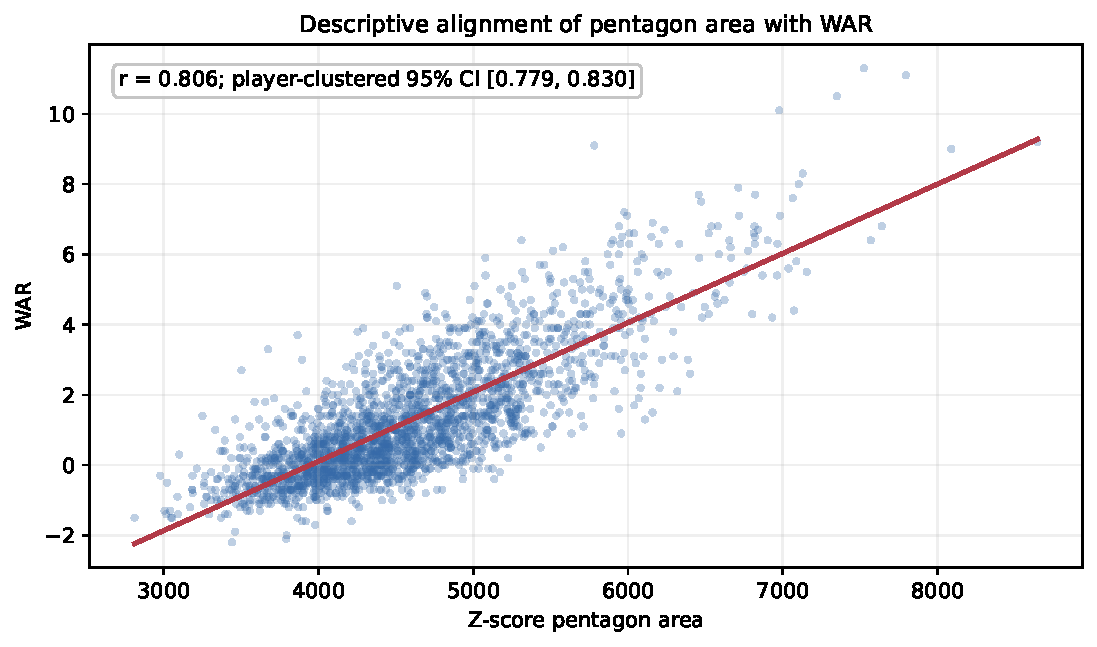
\includegraphics[width=0.78\linewidth]{figures/figure1_alignment_revised.pdf}
\caption{Pentagon area (Z-score encoding) vs.\ WAR over 2{,}309 season-rows ($r=0.806$; player-clustered 95\% CI $[0.779,0.830]$). This is a shared-input descriptive alignment, not independent validation.}
\label{fig:scatter}
\end{figure*}

Four observations follow. First, Z-score averaging has the strongest descriptive alignment with all three metrics, with PCA close behind and the JointVAE lower. This result favors the transparent baseline for the present purpose, but it does not show that learned encodings are generally inferior. Second, although Z-score's and PCA's marginal confidence intervals in Table~\ref{tab:corr} overlap substantially, a paired bootstrap on the same player resamples---which accounts for the fact that all three encodings are computed on the same players and are themselves highly correlated with each other---shows Z-score's edge over PCA is small (0.01--0.02 in $r$) but statistically significant for all three metrics, with a larger, likewise significant gap to JointVAE (0.05--0.16); so the ordering in Table~\ref{tab:corr} is not an artifact of sampling noise, even though eyeballing the marginal intervals alone would suggest otherwise. Third, the observed ceiling near $r \approx 0.8$ versus WAR is consistent with equal weighting across dimensions and with the different construction of WAR; it should not be interpreted as a geometry-independent theoretical limit. Fourth, recomputing area under every axis permutation yields narrow correlation bands for all three encodings ($r$ vs.\ WAR: Z-score $[0.79, 0.82]$, PCA $[0.78, 0.81]$, JointVAE $[0.74, 0.76]$; comparable bands hold for wRC+ and OPS), although individual rankings can remain unstable. Notably, PCA is the most permutation-sensitive of the three encodings, both in absolute terms and as a fraction of its own correlation, so Z-score's advantage over the alternatives should be attributed to its higher, significant correlation with value metrics rather than to any special robustness to the pentagon's axis ordering.

\subsection{Prospective Prediction and Temporal Stability}
\label{sec:prospective-results}
Table~\ref{tab:prospective} reports the forecast-safe fixed 2024$\to$2025 test. B2V-only improves MAE over carry-forward by 4.322 points (95\% paired CI $[2.947,5.838]$) and over calibrated wRC+ Ridge by 1.193 $[0.403,2.012]$; against the latter, $R^2$ improves by 0.074 $[0.022,0.122]$ and $\rho$ by 0.059 $[0.002,0.120]$. The MAE gain is about 6\% of the calibrated scalar model's error: statistically distinguishable here, but practically modest. B2V-context also beats scalar-context by 1.154 MAE points $[0.404,1.880]$, and the combined model beats scalar-context by 1.125 $[0.304,1.929]$, showing incremental information after current wRC+ is included. Conversely, combined versus B2V-context is $-0.029$ $[-0.145,0.086]$, and age/PA versus B2V-only is $-0.001$ $[-0.376,0.368]$; neither current wRC+ nor context clearly adds to B2V. Results condition on returning for at least 100 PA and do not show superiority over unavailable constituent statistics.

\begin{table*}[t]
\centering
\caption{Forecast-safe prospective 2025 wRC+ prediction for 358 returning players, trained on 1{,}056 earlier transitions. Brackets are 95\% held-out-player bootstrap intervals. No row is bolded because paired uncertainty, rather than the best point estimate alone, determines comparisons.}
\label{tab:prospective}
\scriptsize
\begin{tabular}{lccc}
\toprule
Model & MAE $\downarrow$ & $R^2$ $\uparrow$ & Spearman $\rho$ $\uparrow$ \\
\midrule
League mean & 22.274 [20.511, 24.003] & $-0.001$ [$-0.016$, $-0.000$] & --- \\
Carry-forward wRC+ & 22.349 [20.514, 24.386] & $-0.102$ [$-0.298$, 0.078] & 0.449 [0.355, 0.535] \\
Calibrated wRC+ Ridge & 19.220 [17.618, 20.892] & 0.206 [0.119, 0.290] & 0.449 [0.355, 0.535] \\
wRC+ + age + PA Ridge & 19.182 [17.576, 20.756] & 0.220 [0.139, 0.294] & 0.463 [0.378, 0.541] \\
B2V Ridge & 18.027 [16.514, 19.681] & 0.280 [0.179, 0.375] & 0.508 [0.423, 0.589] \\
B2V + age + PA Ridge & 18.028 [16.528, 19.634] & 0.288 [0.192, 0.381] & 0.522 [0.438, 0.600] \\
wRC+ + B2V + age + PA Ridge & 18.057 [16.561, 19.654] & 0.286 [0.190, 0.378] & 0.520 [0.435, 0.600] \\
\bottomrule
\end{tabular}
\end{table*}

Using archived globally scaled vectors instead changes B2V MAE only from 18.027 to 18.023 and $R^2$ from 0.280 to 0.280; the largest individual prediction change is 0.794 wRC+ points. Thus the pooled affine transformation has negligible aggregate impact here, but we do not call the archived-vector experiment leakage-free.

\subsection{Temporal Stability}
Table~\ref{tab:stability} shows that reliability increases with PA and is consistently weakest for Defense. Overall Pearson correlations range from 0.586 (Defense) to 0.775 (Plate Discipline); at 100--249 PA they range from 0.459 to 0.719, compared with 0.635 to 0.806 at 500+ PA. Baseball2Vector should therefore be interpreted as a noisy season summary, particularly for low-PA observations, rather than a fixed latent trait.

\begin{table*}[t]
\centering
\caption{Adjacent-season stability by the smaller of PA$_t$ and PA$_{t+1}$. Cells report $n$ pairs; Pearson $r$ [95\% stable-player-cluster bootstrap CI]. Spearman results are saved with the reproducibility artifacts.}
\label{tab:stability}
\scriptsize
\setlength{\tabcolsep}{3.5pt}
\begin{tabular}{lcccc}
\toprule
Dimension & Overall & 100--249 PA & 250--499 PA & $\geq$500 PA \\
\midrule
Contact & 1414; 0.75 [0.72, 0.78] & 507; 0.63 [0.57, 0.68] & 567; 0.76 [0.71, 0.80] & 340; 0.78 [0.71, 0.84] \\
Power & 1414; 0.75 [0.71, 0.78] & 507; 0.58 [0.51, 0.64] & 567; 0.75 [0.69, 0.80] & 340; 0.80 [0.74, 0.85] \\
Plate Discipline & 1414; 0.77 [0.74, 0.80] & 507; 0.72 [0.67, 0.76] & 567; 0.78 [0.74, 0.82] & 340; 0.81 [0.73, 0.86] \\
Defense & 1414; 0.59 [0.53, 0.63] & 507; 0.46 [0.37, 0.54] & 567; 0.61 [0.52, 0.68] & 340; 0.63 [0.55, 0.70] \\
Speed & 1414; 0.64 [0.60, 0.67] & 507; 0.51 [0.44, 0.58] & 567; 0.65 [0.60, 0.71] & 340; 0.69 [0.61, 0.75] \\
\bottomrule
\end{tabular}
\end{table*}

\subsection{Scalar-Matched Profile Diversity}
\label{sec:matched-profile}
Of 2{,}286 stable-ID focal player-seasons, 2{,}080 meet the joint matching rule (802 unique focal and 709 unique comparison players). Reuse is allowed: 516 comparison players are reused, accounting for 90.7\% of matched rows. Same-player adjacent seasons have median distance 0.714 (IQR $[0.541,0.904]$; 95\% CI $[0.696,0.726]$), scalar-matched different players 1.004 ($[0.746,1.289]$; $[0.980,1.025]$), and matched-focal random pairs 1.188 ($[0.892,1.532]$; $[1.161,1.210]$). Scalar-matched minus same-player distance is 0.291 $[0.264,0.317]$; random minus scalar-matched is 0.184 $[0.154,0.211]$. Thus scalar matching removes some, but not most, profile heterogeneity. The fixed illustrative rule selects Isaac Paredes and Salvador Perez (2024): wRC+ 116/117, WAR 3.3/3.3, PA 641/652, and distance 1.797. The distributions, not this example, are the inferential focus.

\begin{figure*}[t]
\centering
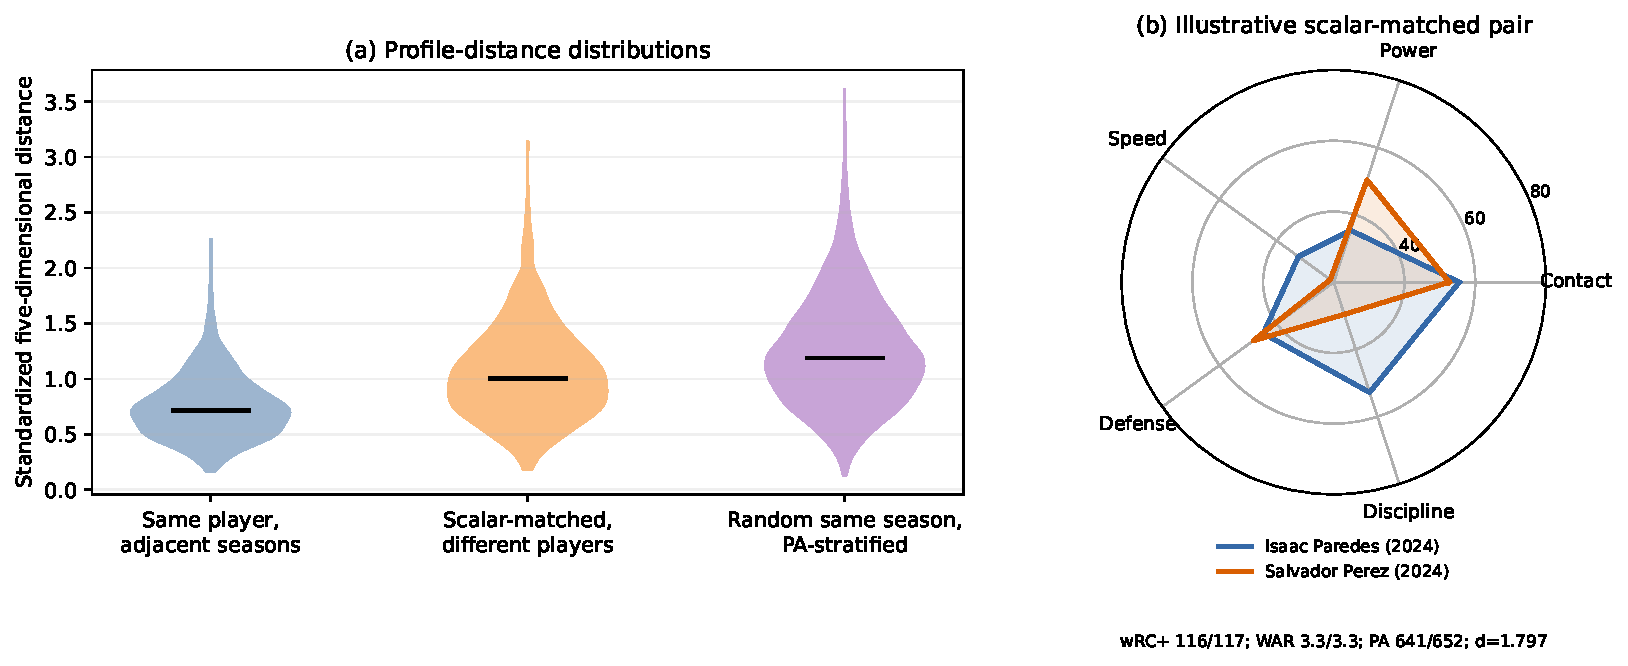
\includegraphics[width=\linewidth]{figures/figure2_profile_diversity_revised.pdf}
\caption{Left: standardized five-dimensional distances for same-player adjacent seasons, deterministically scalar-matched different players, and same-focal PA-stratified random pairs. Black bars mark medians. Right: the verified illustrative scalar-matched pair; displayed metadata and vector scores come from the saved pair row. Scores are cohort-relative, not scouting grades.}
\label{fig:matched-profile}
\end{figure*}

\subsection{Concurrent Dimension-Change Associations}
\label{sec:delta-results}
Conditional on the other concurrent changes, the wRC+ coefficients are Power 3.148 (95\% player-clustered CI $[2.959,3.331]$), Contact 2.168 $[1.966,2.374]$, Plate Discipline 0.704 $[0.521,0.892]$, Defense 0.044 $[-0.103,0.193]$, and Speed $-0.133$ $[-0.273,0.004]$. Shared season statistics partly construct both predictors and target, so Fig.~\ref{fig:delta} reports descriptive partial associations rather than causal exchange rates or training priorities.

\begin{figure}[t]
\centering
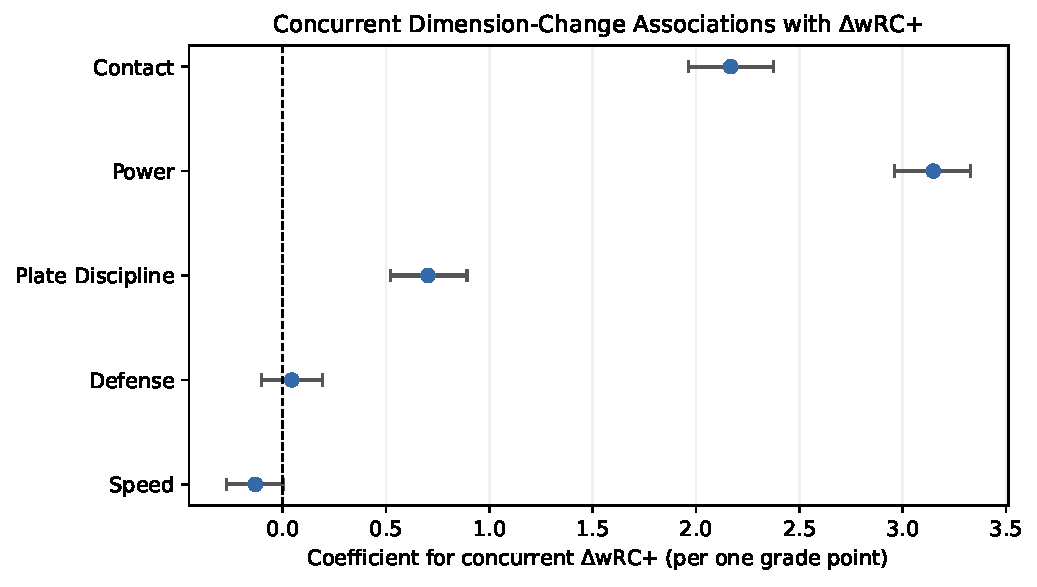
\includegraphics[width=\linewidth]{figures/figure3_delta_association_revised.pdf}
\caption{Linear coefficients for concurrent dimension changes versus $\Delta$wRC+, with 95\% stable-player-cluster bootstrap intervals and a zero reference line. These are descriptive partial associations, not causal exchange rates.}
\label{fig:delta}
\end{figure}

\subsection{Sensitivity Analysis}
Because pentagon area sums adjacent products (Eq.~\ref{eq:area}), it is not permutation-invariant. Population-level correlations vary only within $\pm 0.02$ across orderings, but individual rankings can change substantially as within-player dimension variance increases. Thus, the ``spiky'' profiles for which the full vector is most informative are also those for which radar-chart area is least stable. This finding limits area as a comparison metric and supports using it only as an auxiliary geometric descriptor.

Several planned construction-level checks could not be completed from the archived output: no-/double-shrinkage variants, leave-one-statistic-out encodings, alternative Defense definitions, a constituent raw-statistic predictor, and multi-seed JointVAE stability all require source-level features or model artifacts that are absent. Their absence should be read as unresolved robustness, not as negative evidence. The available results support the usefulness of the released five-dimensional output, but do not identify which upstream design choices are necessary.


\section{Conclusion and Limitations}
\label{sec:conclusion}

Baseball2Vector is an interpretable five-dimensional, cohort-relative season profile with modest incremental next-season information. On the fixed 2024$\to$2025 test, B2V-only outperforms both naive carry-forward and a calibrated current-wRC+ Ridge; adding B2V to scalar context also improves prediction, while adding current wRC+ to B2V context does not. Scalar-matched players remain substantially more distant than the same player across adjacent seasons, showing that the vector preserves profile information discarded by scalar value. The predictive gain over calibrated wRC+ is statistically distinguishable but modest in size and is demonstrated on only one returning-player test year. The results do not validate scouting grades, establish superiority over unavailable raw inputs, or justify causal development recommendations.

\paragraph{Limitations.}
Area correlations remain circular because inputs overlap WAR, wRC+, and OPS, and external construct validity is unestablished. Pooled min--max scores use future extrema; input-season standardization removes this dependence for prediction, but the public display scores remain cohort-dependent. Correlated constituents can double-count signals. Defense is especially problematic because Def contains Fld plus positional adjustment, so their average repeats fielding while mixing position, opportunity, and playing time. The single 2025 test includes only players returning for at least 100 PA, creating survivorship and role-selection bias \cite{nguyen2024}; bootstrap intervals condition on the fixed modeling procedure. Matching reuses comparisons, so its intervals apply to the constructed sample. Missing constituent statistics and JointVAE artifacts prevent raw-input comparison, shrinkage and leave-one-statistic-out checks, alternative Defense construction, and multi-seed latent stability analysis. Concurrent delta coefficients share ending-season information with $\Delta$wRC+ and are not forecasts or causal effects.

\paragraph{Future directions.}
The next priority is a versioned source export with stable IDs and every constituent statistic. It would permit raw-statistic baselines, shrinkage and feature ablations, fielding-only and position-adjusted Defense alternatives, and multi-seed JointVAE evaluation. External validation requires independently verifiable reference data. Prospective tests should span multiple future seasons and model attrition; development claims require subsequently realized changes and adjustment for age, injury, role, position, and playing time. Until then, appropriate use is profile description, comparison, prediction among qualified returners, and hypothesis generation.

%%%%%%%%% REFERENCES
\begin{thebibliography}{99}

\bibitem{mcdaniel2014}
K. McDaniel.
\newblock Scouting explained: The 20--80 scouting scale.
\newblock \emph{FanGraphs Baseball}, 2014. \url{https://blogs.fangraphs.com/scouting-explained-the-20-80-scouting-scale/}.

\bibitem{alcorn2016}
M. A. Alcorn.
\newblock 2vec: Statistic-free talent modeling with neural player embeddings.
\newblock In \emph{MIT Sloan Sports Analytics Conference}, 2016.

\bibitem{heaton2021}
C. Heaton and P. Mitra.
\newblock Learning to describe player form in the MLB.
\newblock \emph{arXiv preprint arXiv:2109.05280}, 2021.

\bibitem{fangraphsSampleSize}
FanGraphs Sabermetrics Library.
\newblock Sample size.
\newblock \url{https://library.fangraphs.com/principles/sample-size/}.

\bibitem{fangraphsDef}
FanGraphs Sabermetrics Library.
\newblock Defensive Runs Above Average (Def).
\newblock \url{https://library.fangraphs.com/defense/def/}.

\bibitem{chadwickRegister}
Chadwick Baseball Bureau.
\newblock Chadwick Register: a repository of baseball player identifiers.
\newblock \url{https://github.com/chadwickbureau/register}.

\bibitem{brown2008}
L. D. Brown.
\newblock In-season prediction of batting averages: A field test of empirical Bayes and Bayes methodologies.
\newblock \emph{The Annals of Applied Statistics}, 2(1):113--152, 2008. \url{https://doi.org/10.1214/07-AOAS138}.

\bibitem{mcshane2011}
B. B. McShane, A. Braunstein, J. Piette, and S. T. Jensen.
\newblock A hierarchical Bayesian variable selection approach to Major League Baseball hitting metrics.
\newblock \emph{Journal of Quantitative Analysis in Sports}, 7(4), 2011. \url{https://doi.org/10.2202/1559-0410.1323}.

\bibitem{jensen2009}
S. T. Jensen, K. E. Shirley, and A. J. Wyner.
\newblock Bayesball: A Bayesian hierarchical model for evaluating fielding in Major League Baseball.
\newblock \emph{The Annals of Applied Statistics}, 3(2):491--520, 2009. \url{https://doi.org/10.1214/08-AOAS228}.

\bibitem{baumer2015}
B. S. Baumer, S. T. Jensen, and G. J. Matthews.
\newblock OpenWAR: An open source system for evaluating overall player performance in Major League Baseball.
\newblock \emph{Journal of Quantitative Analysis in Sports}, 11(2):69--84, 2015. \url{https://doi.org/10.1515/jqas-2014-0098}.

\bibitem{nguyen2024}
Q. Nguyen and G. J. Matthews.
\newblock Filling the gaps: A multiple imputation approach to estimating aging curves in baseball.
\newblock \emph{Journal of Sports Analytics}, 10(1):77--85, 2024. \url{https://doi.org/10.3233/JSA-240744}.

\bibitem{mikolov2013}
T. Mikolov, K. Chen, G. Corrado, and J. Dean.
\newblock Efficient estimation of word representations in vector space.
\newblock {\em arXiv preprint arXiv:1301.3781}, 2013.

\bibitem{kingma2014}
D. P. Kingma and M. Welling.
\newblock Auto-encoding variational Bayes.
\newblock In {\em ICLR}, 2014.

\end{thebibliography}

\end{document}
